% File hicss51.tex
%%
%% Based on the style files for ACL 2015 by 
%% car@ir.hit.edu.cn, gdzhou@suda.edu.cn


\documentclass[10pt]{article}
\usepackage[letterpaper]{geometry}
\usepackage{hicss51}
\usepackage{times}
\usepackage[none]{hyphenat}
\usepackage{url}
\usepackage{latexsym}
%\usepackage{minted}
\usepackage{indentfirst}
\usepackage{graphicx}
%\graphicspath{{images/}}
\usepackage{wrapfig}
\usepackage{todonotes}
\usepackage{hyperref}
\usepackage[utf8]{inputenc}
\newcommand{\sansserifformat}[1]{\fontfamily{cmss}{ #1}}%

%\setlength\titlebox{5cm}


% You can expand the titlebox if you need extra space
% to show all the authors. Please do not make the title box
% smaller than 5cm (the original size).



\title{Open Source Intelligence - Development of a Trend Radar utilizing a Systematic Literature Review}

\author{Franz Kayser \\
  ESG \\
  {\underline{ franz.kayser@esg.de}} \\\And
  Thomas Mayer \\
  ESG  \\
  {\underline{ thomas3.mayer@esg.de} }\\\And 
  Michael Bücker \\
  FH Münster -- University of Applied Sciences\\
  {\underline{michael.buecker@fh-muenster.de}} \\}

\date{}

\begin{document}
\maketitle
\begin{abstract}
    Open Source Intelligence (OSINT) is currently experiencing an intensive discourse,
    heightened since the Russian invasion of Ukraine. However, despite numerous attempts
    at standardized definitions, the intelligence discipline remains ambiguous. This paper
    introduces a practice-validated OSINT trend radar, categorizing technologies by maturity,
    intelligence cycle phase, and use case. Serving as a profound knowledge base and tool for
    identifying research gaps, the radar emerges from a structured design process. Sixty
    studies underwent categorization and validation through expert interviews,
    revealing the absence of a comprehensive, autonomous third-generation OSINT
    system in Germany. Technological gaps, especially in the planning and direction and
    dissemination and integration phases, are evident. Although intelligent support
    technologies were identified, practical implementation lags behind theory. The human
    factor therefore remains central to the OSINT process. Future research should thus
    prioritize developing applications for underserved phases, probing reasons for limited
    widespread implementation of proven applications, with emphasis on legal, ethical,
    political, and social parameters.
\end{abstract}

\section{Introduction}

OSINT is a currently more debated research field than ever before. Obtaining intelligence
from publicly available data \cite{DosPassos.2017} has become undeniably important since the
Russian invasion of Ukraine in 2022. The real-time analysis of social media in particular has
brought highly relevant insights to light \cite{Hatfield.2023, SmithBoyle.24.07.2023}. However, despite
numerous attempts to define OSINT (e.g. \cite{Hwang.2022, PastorGalindo.2020, Yogish.2021}),
the concept remains controversial to this day \cite{Ghioni.2023, Ish.2022,Williams.2018}.
This is not least because every definition of OSINT is subject to the advances
in computer and data sciences, which continuously produce improvements in (intelligent)
collection and analysis possibilities \cite{Ghioni.2023, Williams.2018}. This is
accompanied by numerous new open means of communication, which have caused a veritable
"information explosion" \cite{DosPassos.2017, Hwang.2022, Yogish.2021}.
Data sources that were originally reserved for the defense and intelligence services are
now publicly accessible \cite{Hwang.2022, Williams.2018}. The understanding of
intelligence thus changed completely \cite{Dokman.2020}.

To date, there has been a lack of fundamental scientific publications to penetrate
the subject area \cite{HerreraCubides.2020} and address its rapid
developments \cite{Ghioni.2023, Williams.2018}. In particular, there is a shortage of
studies that identify the technologies behind OSINT and determine their characteristics.
The question of whether autonomous third-generation OSINT systems \cite{PastorGalindo.2019, PastorGalindo.2020} exist
has not yet been clarified \cite{Ghioni.2023, PastorGalindo.2020,Yogish.2021}.
Moreover, the majority of studies focus exclusively on the OSINT trend area "cyber
security" \cite{Hwang.2022, PastorGalindo.2019, Yogish.2021}. The literature thus failed to
cover the topic in its entirety. Important use cases of OSINT have
therefore not yet been researched \cite{AlKilani.2021, Dokman.2020, Ghioni.2023}.
In addition, supplementary qualitative field research is absent to contrast theory with
the corresponding practical implementation. Although OSINT has a major impact on topics
such as security and defense, there is a lack of insight into these sectors \cite{HerreraCubides.2020, PastorGalindo.2019}.
This paper is hence dedicated to answering the research question:
\textit{How can the current trends in OSINT in the form of the technologies used and their
    characteristics, in particular the maturity level and the use case, be presented in a
    trend radar and validated by experts within the security sector?}

The thereby aim is to identify the technologies used in OSINT applications and to present
them systematically in a trend radar, according to their characteristics. In this way, a well-founded knowledge base will
be compiled, and practice-relevant research gaps will be identified for a coordinated examination
of the research field. The study follows the "Design Science Research Model" (DSRM)
\cite{Peffers.2007}.  First, the relevant literature on OSINT will be analyzed and classified
through a systematic literature review \cite{Webster.2002}. Second, the OSINT technologies and
their characteristics identified will be visualized in the form of a trend radar. The radar
will then be validated using systematizing interviews \cite{Bogner.2014} conducted with
experts in the security sector. Finally, the interviews will be evaluated using a
qualitative content analysis [21].

\section{Theoretical Background}

The domain of OSINT is continuously expanding due to the ongoing improvements of
collecting and analysis possibilities \cite{AlKilani.2021, Ghioni.2023, Williams.2018}. In
addition, the new means and methods of communication associated with advances in information
and communication technology have turned OSINT into a complex discipline
\cite{AlKilani.2021, Benes.2013, Chen.2012, Williams.2018}.

\subsection{Open Source Intelligence (OSINT) and its Components}

One of the earliest and still frequently referenced definitions \cite{DosPassos.2017}
was published by NATO in 2001. OSINT according to this definition is information that has been
deliberately discovered, discriminated, distilled, and disseminated to a select audience,
[...], in order to address a specific question. OSINT, [...] thus applies the proven
process of intelligence to the broad diversity of open sources [...] and creates
intelligence [23]. However, today the discipline is no longer seen as a purely governmental
matter. Private research institutions and organizations \cite{Bohm.2021,Mercado.2005} are
also massively driving the development of such systems, e.g. for competitive analyses or marketing activities
\cite{AlKilani.2021, Dokman.2020,Ghioni.2023}. The focus is thereby shifting to
developing OSINT into a robust, autonomous solution (referred to as third-generation) \cite{Billings.1997,PastorGalindo.2019,Schaurer.2010}.
The starting point for all OSINT activities thereby lies in data. Data forms the basis of the
analysis and the conclusions derived from it \cite{Gibson.2016}. In this context, Open Source Data (OSD)
refers to non-processed \cite{DosPassos.2017}, general raw data that is openly available
\cite{Burke.2007} as well as legally and ethically accessible
\cite{Schaurer.2010, NorthAtlanticTreatyOrganization.2001}. Before intelligence can be obtained
from OSD, they must undergo a preparation process that includes filtering, validation and
summarization \cite{DosPassos.2017, NorthAtlanticTreatyOrganization.2001}. The result of this
data organization \cite{Schaurer.2010} is referred to as Open Source Information (OSINF). It provides the basis for the
resulting intelligence creation \cite{DosPassos.2017,Schaurer.2010}.

\subsection{Intelligence and Intelligence Cycle}

The core task of OSINT is to generate intelligence \cite{Hwang.2022,Dokman.2020}
in terms of a profound basis for decision-making
\cite{Breakspear.2013,May.2020}. The generation process of such an intelligence product
is also referred to as the intelligence cycle \cite{HerreraCubides.2020, CentralIntelligenceAgency.1987}.
It represents the central element of every intelligence discipline \cite{Reuser.2017,Dokman.2020}. The link between the phases is that
the result of the preceding phase serves as input for the subsequent phase
\cite{JointChiefsofStaffU.S.Army.2013,Pellissier.2013}. Furthermore, the individual phases are also continuously
iterated due to the fulfillment of previous requirements and new demands\cite{Gibson.2016}.
Today, to represent external influences or the
assignment of responsibilities \cite{Lowenthal.2020,Phythian.2013,Johnston.2005}, numerous
variations can be found \cite{Bohm.2021,Reuser.2017}. The
Intelligence Cycle should therefore be seen less as a guideline and more as an informal
coordination element\cite{Hwang.2022}.
In 2013, the JCS segmented the cycle into 6 phases [32] (see Fig \ref{fig: intelligence cycle}).

\begin{figure}[h]
    \centering
    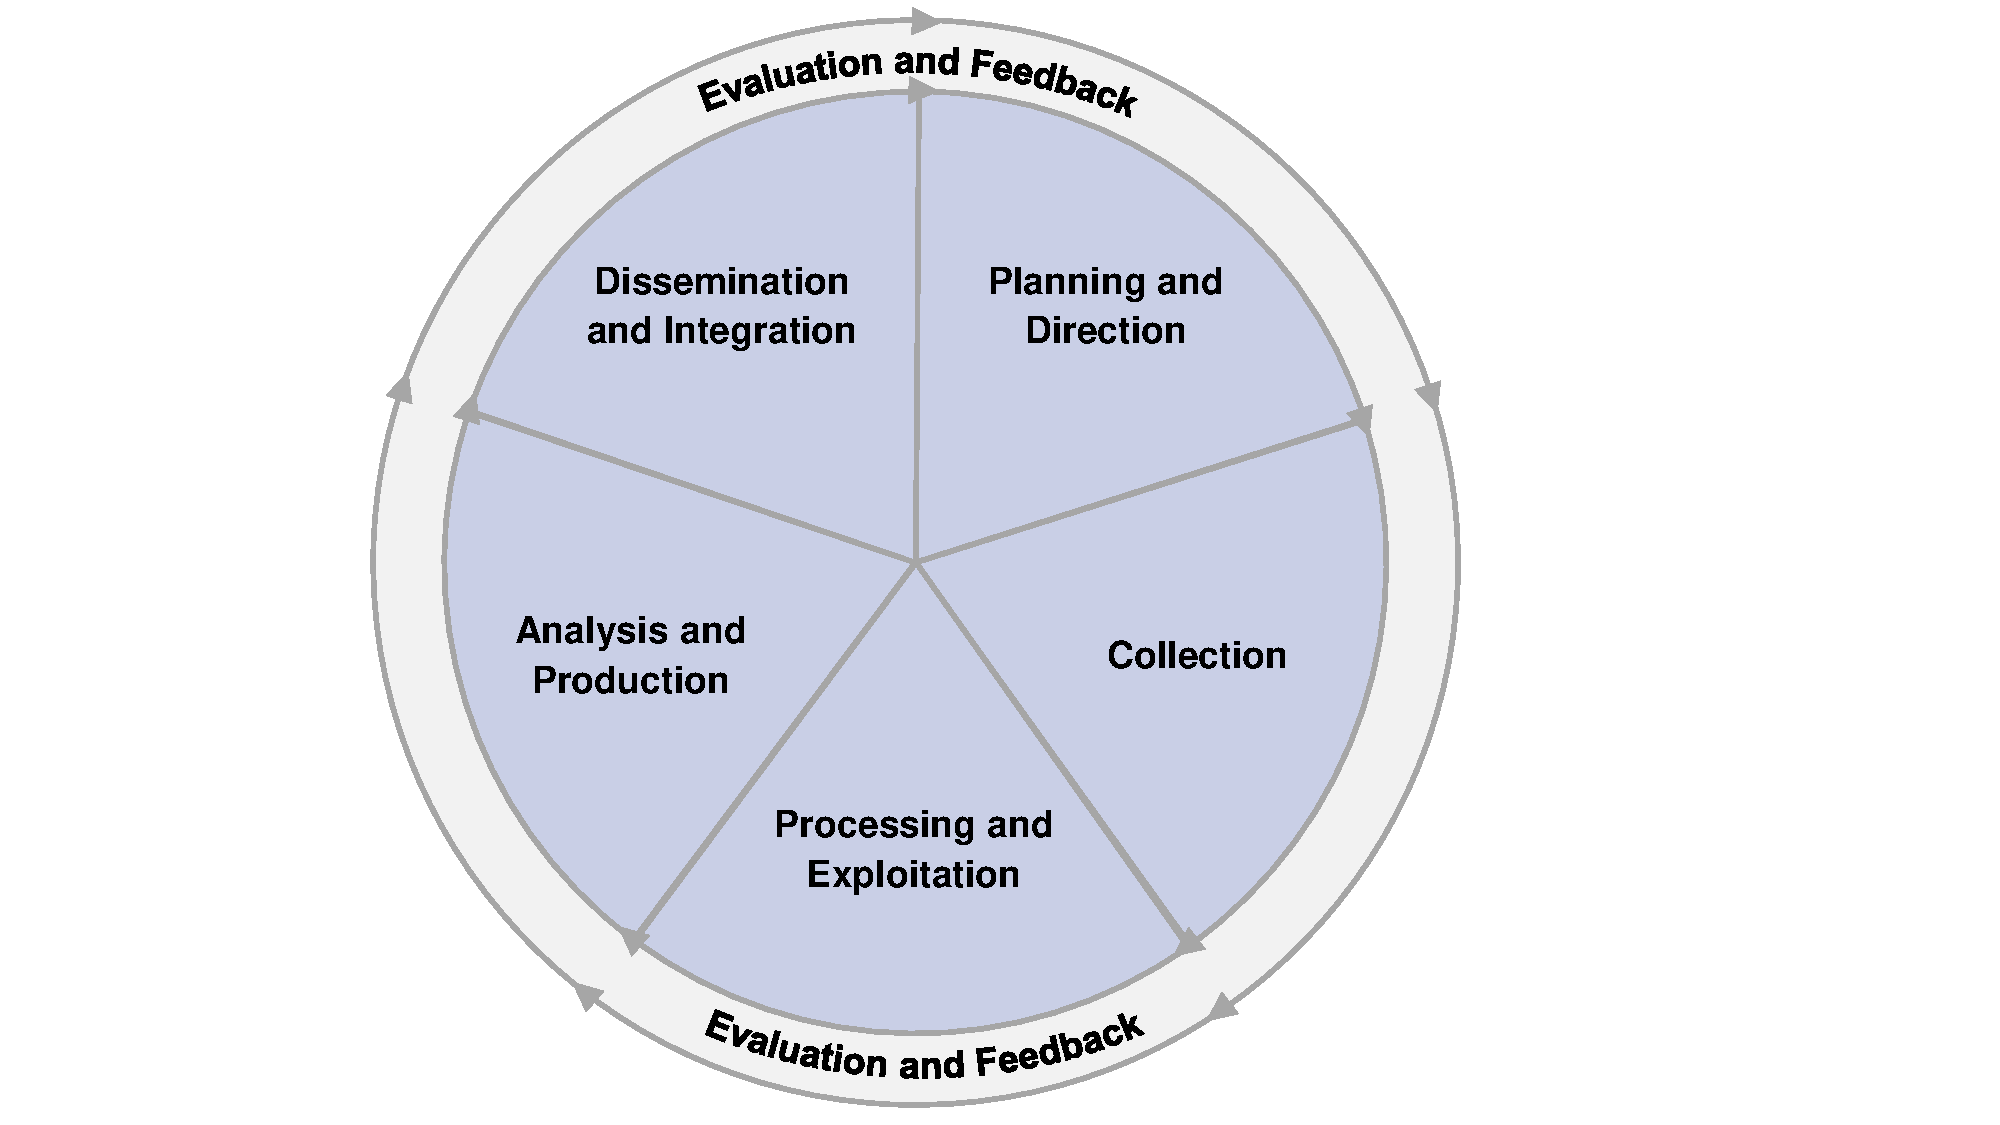
\includegraphics[clip,width=0.9\linewidth]{crop_Intelligence Cycle}
    \caption{Intelligence Cycle, according to \cite{JointChiefsofStaffU.S.Army.2013}}
    \label{fig: intelligence cycle}
\end{figure}

The planning and direction phase combines the identification, definition and prioritization
of the requirements for the cycle. It is also responsible for developing and monitoring the activities
required to achieve these \cite{DepartmentoftheArmy.2012, JointChiefsofStaffU.S.Army.2013, DepartmentoftheArmy.2012}.
The collection phase refers to the gathering of raw data \cite{CentralIntelligenceAgency.1987}.
The core of this phase consists of the iterative repetition of research
\cite{NorthAtlanticTreatyOrganization.2001} to make the query more precise with each run
\cite{PastorGalindo.2020}. The processing and utilization phase involves condensing
these data volumes into action-relevant information
\cite{DirectorofNationalIntelligence.2011, JointChiefsofStaffU.S.Army.2013, PastorGalindo.2020}.
Analysis and production refers to the synthesis of the information obtained into a
user-oriented, timely and accurate intelligence product
\cite{DepartmentoftheArmy.2012, Hwang.2022, NorthAtlanticTreatyOrganization.2001}.
The final phase consists of handing over the finished product to the "customer" in a
usable form \cite{CentralIntelligenceAgency.2023, DepartmentoftheArmy.2012, Williams.2018}.
Evaluation and feedback are not to be regarded as individual phases
but take place continuously throughout the entire cycle. The aim is to achieve progressive optimization
\cite{DirectorofNationalIntelligence.2011, JointChiefsofStaffU.S.Army.2013, NorthAtlanticTreatyOrganization.2001}.

\subsection{Previous Studies}

Eight previous, publicly accessible literature reviews can be identified
concerning OSINT. In 2017, Dos Passos \cite{DosPassos.2017} showed how big data and data science can
make the decision-making process more useful and effective. Pastor-Galindo et al. then described
the current state of OSINT in 2019 \cite{PastorGalindo.2019} and 2020 \cite{PastorGalindo.2020}
focusing on services and techniques to improve cybersecurity. Moreover, they are responsible
for the first and only rudimentary mapping of OSINT trends. They observed that OSINT is used in
social opinion and sentiment analysis, cybercrime and organized crime, as well as cybersecurity and cyberdefence.
Two further literature reviews were published in 2020. García Lozano et al. \cite{GarciaLozano.2020} identified
methods for computer-assisted veracity assessment of public information.
Herrera-Cubides et al. \cite{HerreraCubides.2020} investigated how the production of
research and educational materials has developed. They concluded that
the number of OSINT publications is lower compared to other trending topics. In 2021,
Yogish and Krishna \cite{Yogish.2021} explored the state of implementation and use of
Artificial Intelligence (AI) technologies in the context of cybersecurity. The result of this
study showed that Machine Learning (ML), pattern recognition and Natural Language Processing
(NLP) can simplify OSINT given increasing data volumes. In the following year, Hwang et al.
\cite{Hwang.2022} investigated security threats and cybercriminality in the context of OSINT misuse.
In 2023, Ghioni et al. \cite{Ghioni.2023} then examined the political, ethical, legal and social implications of
OSINT in conjunction with AI. They discovered that there is still no framework
for addressing these. They also found that third-generation OSINT is still in its early
stages and that human components cannot yet be replaced.


\section{Research Methodology}

The structure of the study is based on the iterative DSRM \cite{Peffers.2007}. It is a theory-based
research paradigm for developing an explicitly applicable solution, in the form of an innovative artifact,
\cite{vomBrocke.2020b}, solving a (practical) problem \cite{Peffers.2007,Hevner.2004}. The model is therefore ideally suited to
create the trend radar. It consists of six successive activities (see Fig. \ref{fig: DSRM}) \cite{Peffers.2007}.
Moreover, the first three evaluation steps according to Sonnenberg and vom Brocke \cite{Sonnenberg.2012}
were applied to continuously evaluate the design process.

\begin{figure*}[thb]
    \centering
    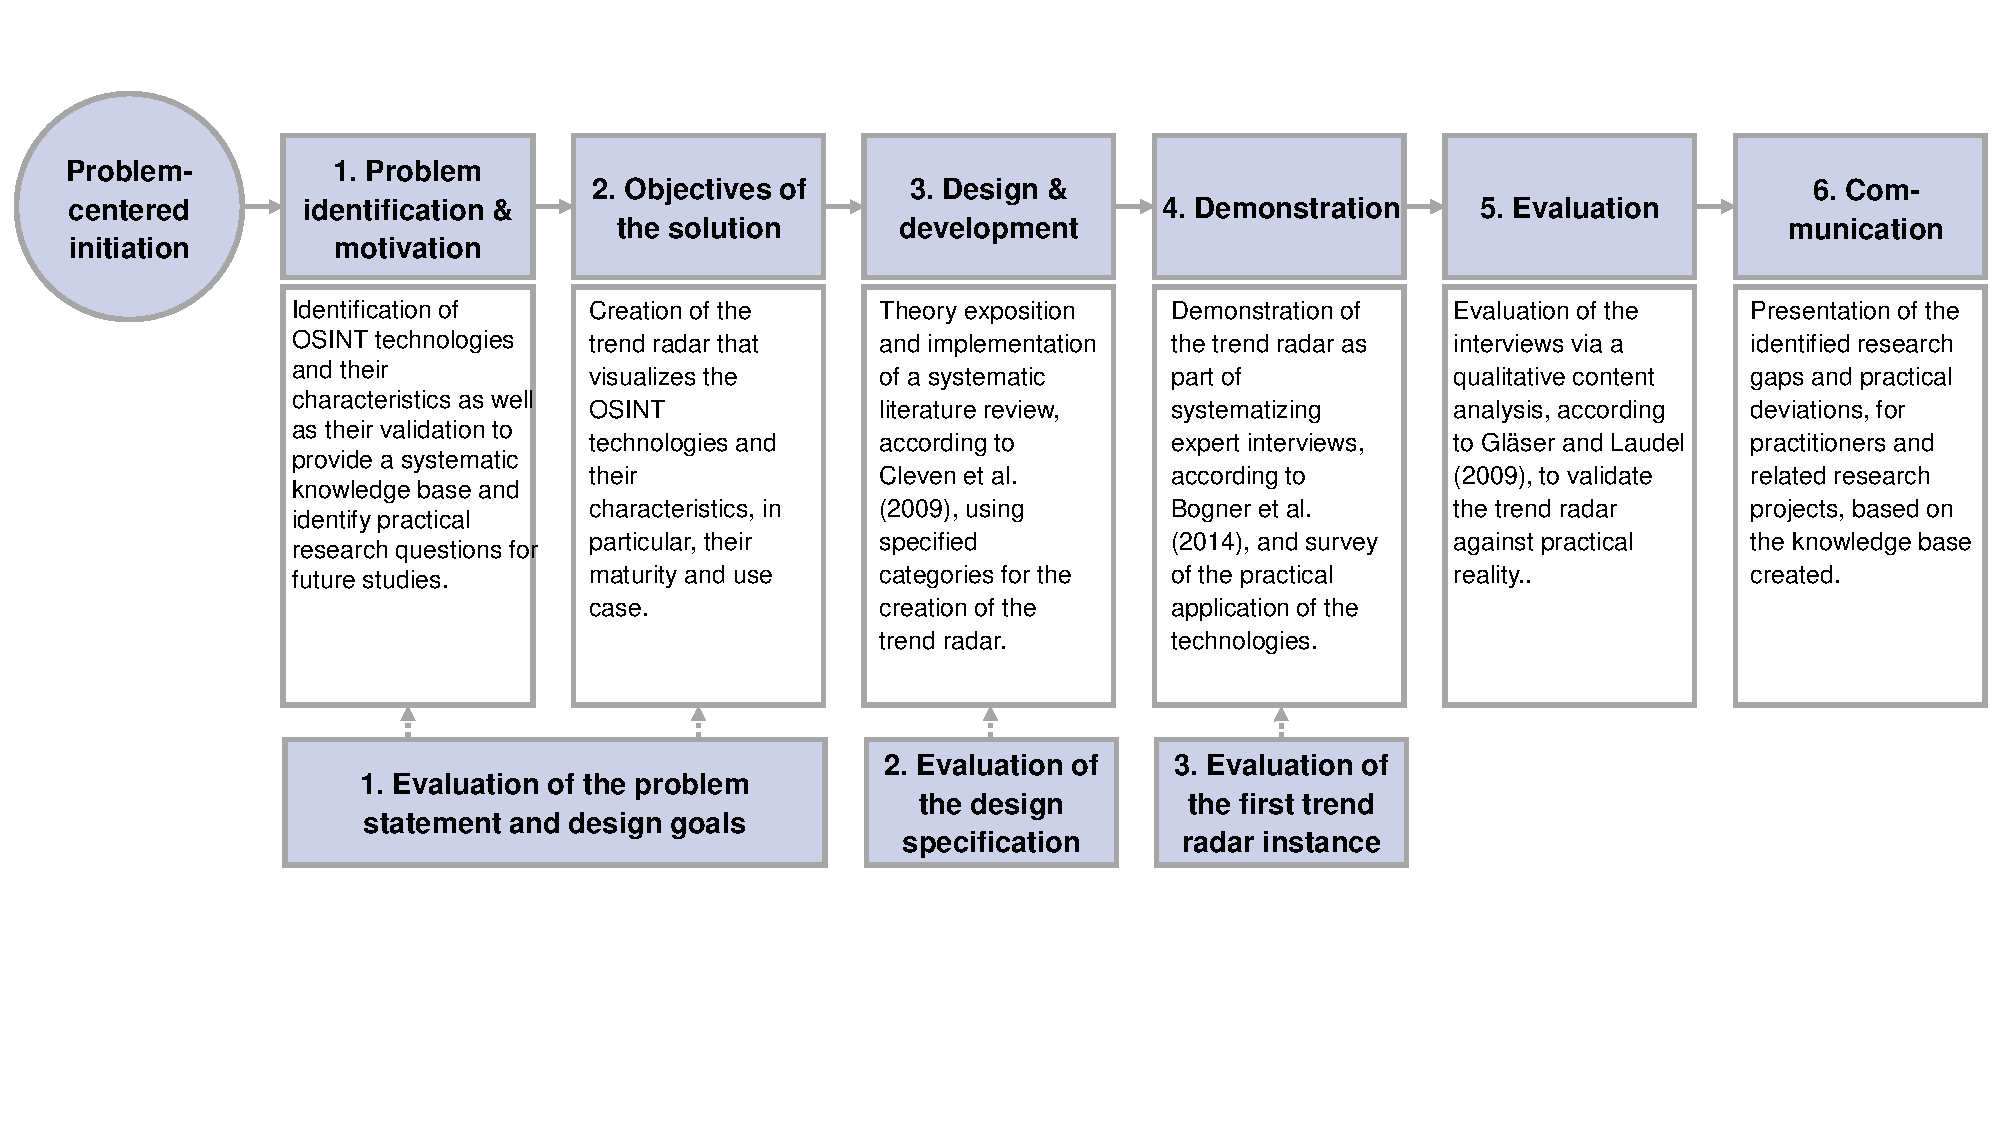
\includegraphics[width=\textwidth]{crop_DSRM}
    \caption{Design Science Research Model (DSRM)}
    \label{fig: DSRM}
\end{figure*}

\subsection{Problem Identification and Motivation}

First, the research problem must be defined and the benefits of the solution explained (see chapter Introduction).

\subsection{Design Objectives of the Solution}

The next step is to define the design objectives of the solution. The
objectives can be divided into two content-related objectives (CO) and
two formal objectives (FO). CO1 requires the trend radar to follow a procedural
structure that reflects the process of generating intelligence. This will allow a structured mapping of the
identified technologies according to their use. In doing so, any
research gaps that become apparent can be directly assigned to the
respective phase. It will thus be possible to verify if a third-generation OSINT system exists. As CO2, it was defined that the key
characteristics, in particular the maturity level of the technologies
and their use cases, must be taken into account. The maturity level of
the technologies makes it possible to determine the respective research status.
Through the use cases, the research directions can be
revealed. As FO1, it was determined that the trend radar must follow
a simple structure to enable the immediate identification of research gaps. In addition,
the radar should have a high degree of standardization to be
transferable to other intelligence gathering disciplines in later
studies. As FO2, it was decided that the trend radar should be continuously expandable to capture the high field dynamics.

\subsection{Evaluation of the Problem Statement and Design Objectives}

In the theoretical background section, the main definitions, in
particular, the intelligence cycle, which serves as a basis for the
development of the trend radar ("suitability"), were presented. Moreover,
the presentation of previous research work showed that there
is still a lack of broad-based studies examining OSINT. Both the
relevance of the research question and the suitability of the
design objectives are thus underpinned \cite{Sonnenberg.2012}.

\subsection{Design and Development}

The third activity involves the creation of the artifact. For this
purpose, the relevant literature on OSINT was analyzed through a
systematic literature review \cite{Cleven.2009}. To clearly define the scope of the literature
review, Cooper's taxonomy \cite{Cooper.1988} was used. Subsequently, classification
categories were defined to establish concept matrices \cite{Webster.2002},
to systematically analyze the researched literature. To achieve a high degree of standardization,
general categories were defined for each phase of the intelligence
cycle. The evaluation and feedback phase was not treated separately due
to its iterative nature.

The following six categories were defined for the collection
phase: "use case", "data", "process", "technology", "technology
complexity" and "maturity level". First, the area of application
of the technologies was recorded under the use case. The
category data reveals the composition of the data foundation. It is further subdivided
into the data type to record the formats and
the source to show the origin of the data. The category
process is used to determine the degree of automation of the technologies. For this purpose, the following
four levels were defined: manual, semi-automated, automated,
\cite{Duncheon.2002} fully automated/autonomous \cite{Billings.1997,Endsley.1999}.
To improve categorization, the ten levels of automation \cite{Sheridan.1978,Parasuraman.2000}
were used. The fourth category serves to capture the technologies, defined
as "the totality of material and immaterial means available for
the input, output, conversion, transmission and storage of information" \cite{Bleck.2004}.
The fifth category evaluates the complexity of the technologies
examined. The three subcategories
"Volume" \cite{OLeary.2012}, "Variety" and "Velocity" were used \cite{Elgendy.2014,Russom.2011,Singh.2012}.
Variety is further subdivided according to the data structure (structured \cite{Lin.2018},
semi-structured and unstructured \cite{Katal.2013,Praveen.2020}) \cite{OLeary.2012}. Velocity,
is further subdivided into the levels "Batch" \cite{Carbone.2015}, "Near Real-Time"
\cite{Stankovic.1990,Gomes.2021} and "Real-Time" \cite{Stankovic.1990}. The sixth category reflects the
maturity level of the technologies used, based on the three macro-maturity phases of the
German Federal Trend Radar: innovation phase, prototype phase and
market establishment phase \cite{Stich.2022}.

For the remaining phases the categories use case, process,
technology, technology complexity and maturity level
were likewise defined. However, the complexity within the remaining
phases is measured based on the underlying analysis, in
ascending order: descriptive analysis, diagnostic analysis, predictive
analysis, prescriptive analysis \cite{Delen.2013,GartnerGmbH.2012}.

After defining the classification criteria, the literature research
was carried out (Fig. \ref{fig: Literature review}). A search string based on
general terms for the highest possible number of hits was determined. Only studies
with full access were considered. As the number of publications
increased significantly between 2020 and 2023, the period was reduced
to these years to ensure the most up-to-date coverage possible.
The studies were downloaded on 05.06.2023. The
SQR3 method \cite{Robinson.1970} was applied for the systematic analysis and further
delimitation. Altogether 60 studies were categorized.

\begin{figure}[t]
    \centering
    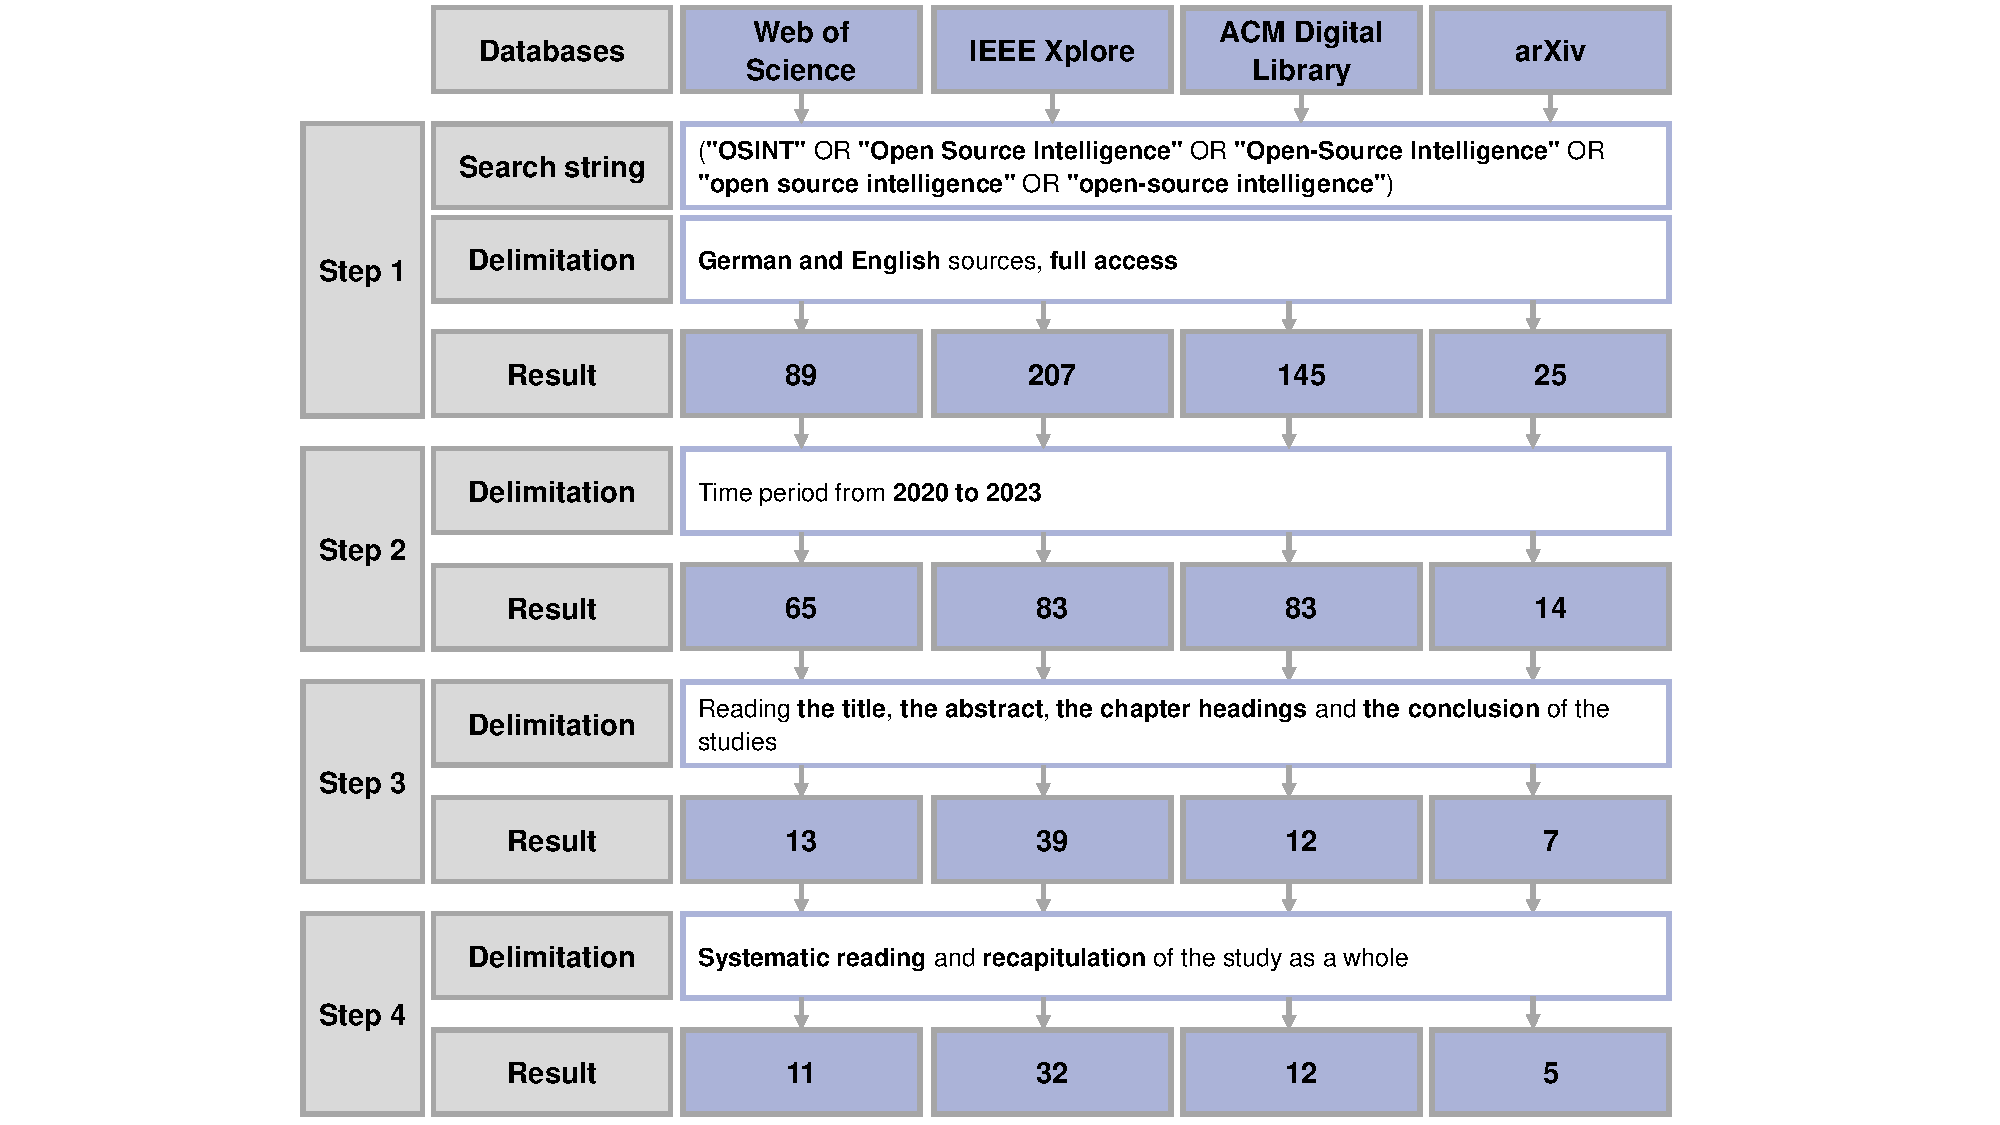
\includegraphics[width=0.6\textwidth]{crop_Kategorisierungskriterien und Literraturreviewaufbau}
    \caption{Literature review}
    \label{fig:LiteratureReview}
\end{figure}

For categorization, a dedicated Excel spreadsheet was created per
Intelligence Cycle phase and the OSINT technologies and their
characteristics were methodically recorded \cite{Cleven.2009, Webster.2002}. The identified
technologies were then grouped according to relations in an
additional column (see Repository X). Afterward, the categorization was
verified using a "Python" script (see Appendix A). This
queries the occurrence of predefined keywords in the included papers.
Afterward, the trend radar was created based on the verified concept matrices.

\subsection{Evaluation of the Design Specifications}

The intelligence cycle as the basis of the trend radar provides a
structured overview ("clarity") \cite{Breakspear.2013}. This
fulfills the requirement of an intuitively understandable illustration
("understandability") for ensuring a simple extraction ("simplicity")
of technologies and research gaps. Furthermore, the other intelligence
disciplines are also derived from the cycle, which enables a later
application to these ("applicability"). By aligning the
architecture of the radar with the federal government's trend radar
\cite{Stich.2022}, a proven, robust, user-friendly
design ("user-friendliness") with an appropriate level of detail
("level of detail") is used. Only the categories use case, technology and
degree of maturity were therefore illustrated. Moreover, with the concept matrices, a
template is used to constantly update the radar. Particular attention
was paid to the general validity of the categories to achieve
the highest possible degree of standardization ("generality").
Furthermore, a verification of the categorization was carried out ("internal consistency").
The decisive evaluation criteria \cite{vomBrocke.2020b} are thus fulfilled.

\subsection{Demonstration}

Next, the trend radar was demonstrated via guideline-based,
systematizing expert interviews \cite{Bogner.2014, Glaser.2009, Meuser.1991}.
Especially in less structured and sparsely linked subject areas, the method
enables dense data collection \cite{Bogner.2014,Meuser.1991}. Additionally,
it is suitable in cases where access to the social field is limited \cite{Bogner.2002c, Glaser.2009}.

The experts (Tab. \ref{tab: experts}) were selected according to the method of
theoretical sampling \cite{Glaser.1967,Eisenhardt.1989}. It was specified that only experts in
Germany should be interviewed to validate the trends in this
country. It was also determined that at least one expert each
from a security authority, the security industry and a
start-up would be selected to capture different points of
view. A "prestigious" company position is seen as a reliable
guarantee that the respondents possess research-relevant knowledge \cite{Bogner.2002b}.

\begin{table}[htbp]
    \label{tab:experts}
    \caption{Interviewed experts}
    \begin{tabular}{|p{0.25\linewidth}|p{0.55\linewidth}|p{0.05\linewidth}|}
        \hline
        \textbf{Organization} & \textbf{Position}                                                         & \textbf{ID} \\
        \hline
        Industry/ Authority   & Senior Intelligence Consultant                                            & E1          \\
        \hline
        Industry/ Authority   & Referent Corporate Security                                               & E2          \\
        \hline
        Authority             & In-House Senior Consultant                                                & E3          \\
        \hline
        Start-up              & Co-Founder, Managing Director of a German start-up, for an OSINT platform & E4          \\
        \hline
    \end{tabular}
\end{table}

The qualitative data collection that followed was carried out using
semi-structured interviews. These are particularly suitable for
revealing the underlying relationships of a theory \cite{Bogner.2014}. The
questionnaire used is based on the structure of the Intelligence Cycle.
At the beginning of the interview, the trend radar was presented.
To compare it with the respondents' practical experience, first, open questions
were asked for each phase. These reduce the influence of
subjectivity \cite{Saunders.2012}. Exploratory questions were added to direct the flow of conversation
\cite{Saunders.2012}. Thirs, specific closed questions for targeted follow-up
queries were asked \cite{Saunders.2012}. The interviews lasted up to one hour, with a maximum of three
main questions for each phase \cite{Bogner.2014} (see Respository X). The questionnaire
was pilot-tested with a domain expert. The interviews were conducted online.

\subsection{Evaluation of the First Instance of the Trend Radar}

The demonstration of the trend radar confirmed its intuitive
comprehensibility ("ease of use"). It was also perceived by the
practitioners as a useful tool for providing an overview of OSINT
technologies ("effectiveness"). In addition, they confirmed its
completeness ("completeness") and internal consistency ("consistency")
(cf. expert E1, 14.08.2023; expert E3, 28.07.2023; expert E4,
02.08.2023). The trend radar thus proved to be a
suitable instrument for identifying research gaps and for serving as a guideline to practitioners
("fidelity with real world phenomenon"). The essential evaluation
criteria \cite{Sonnenberg.2012} are thus demonstrably fulfilled.

\subsection{Evaluation}

The evaluation was carried out using a qualitative data analysis \cite{Glaser.2009}.
It extracts, synthesizes and structures the information contained in the interviews
using a predefined search grid. This enables the targeted
extraction and summarization of relevant, cross-interview information
according to a "top-down approach" \cite{Bogner.2014, Glaser.2009}.

First, the recorded interviews were transcribed. Second, the software
MAXQDA \cite{MAXQDA.19.07.2023} was used for the subsequent analysis.
The categorization system was therefore established as grid within MAXQDA
(see repository X). The categories of the first level correspond to
the individual phases of the intelligence cycle. The categories of the
second level allow a classification of whether the experts express
themselves in support of or in contradiction to the theory. The
categories of the third level reflect the identified use cases.
As many of the experts' statements were general, the
category "general statements" was added. The categories
of the fourth level reflect the individual technologies classified
under them. Altogether, 257 statements were categorized in this way. Examples of the coding
procedure can be found in Tab. \ref{tab:coding}.

\begin{table*}[htbp]
    \caption{Coding examples}
    \label{tab:coding}
    \begin{tabular*}{\textwidth}{|p{0.12\linewidth}|p{0.12\linewidth}|p{0.12\linewidth}|p{0.12\linewidth}|p{0.39\linewidth}|}
        \hline
        \textbf{Level 1} & \textbf{Level 2} & \textbf{Level 3} & \textbf{Level 4} & \textbf{Transcript example} \\
        \hline
        Collection phase & Theory- supporting & General statement & "web crawler" and/or "web scraper" & And precisely because there are so many, so simple ways to create web crawlers and web scrapers, [...]"(Cf. expert E1, 14.07.2023) \\
        \hline
        Analysis and production phase & Theory- contradictory & Security & AI, ML, DL & "Deep learning, machine learning, artificial intelligence, in some places, I don't know anyone who has built in a random forest anywhere [...]" (cf. E3, 02.08.2023) \\
        \hline
    \end{tabular*}
\end{table*}

\subsection{Communication}

The research results are communicated in the form of this study.
A new iteration, proceeding from this chapter, is therefore not
carried out.

\section{Results}

The trend radar (\ref{fig:trendradar}, \ref{fig:trendradarexplanation}) is read from the outermost to the innermost.
Each fifth of the cycle represents an Intelligence Cycle phase. Subdivisions indicate
phase-specific use cases, while color gradations show maturity levels. Numbered black
and white dots denote grouped technologies, presented in a boxplot-like format reflecting
varying maturity levels.

\begin{figure*}[thb]
    \centering
    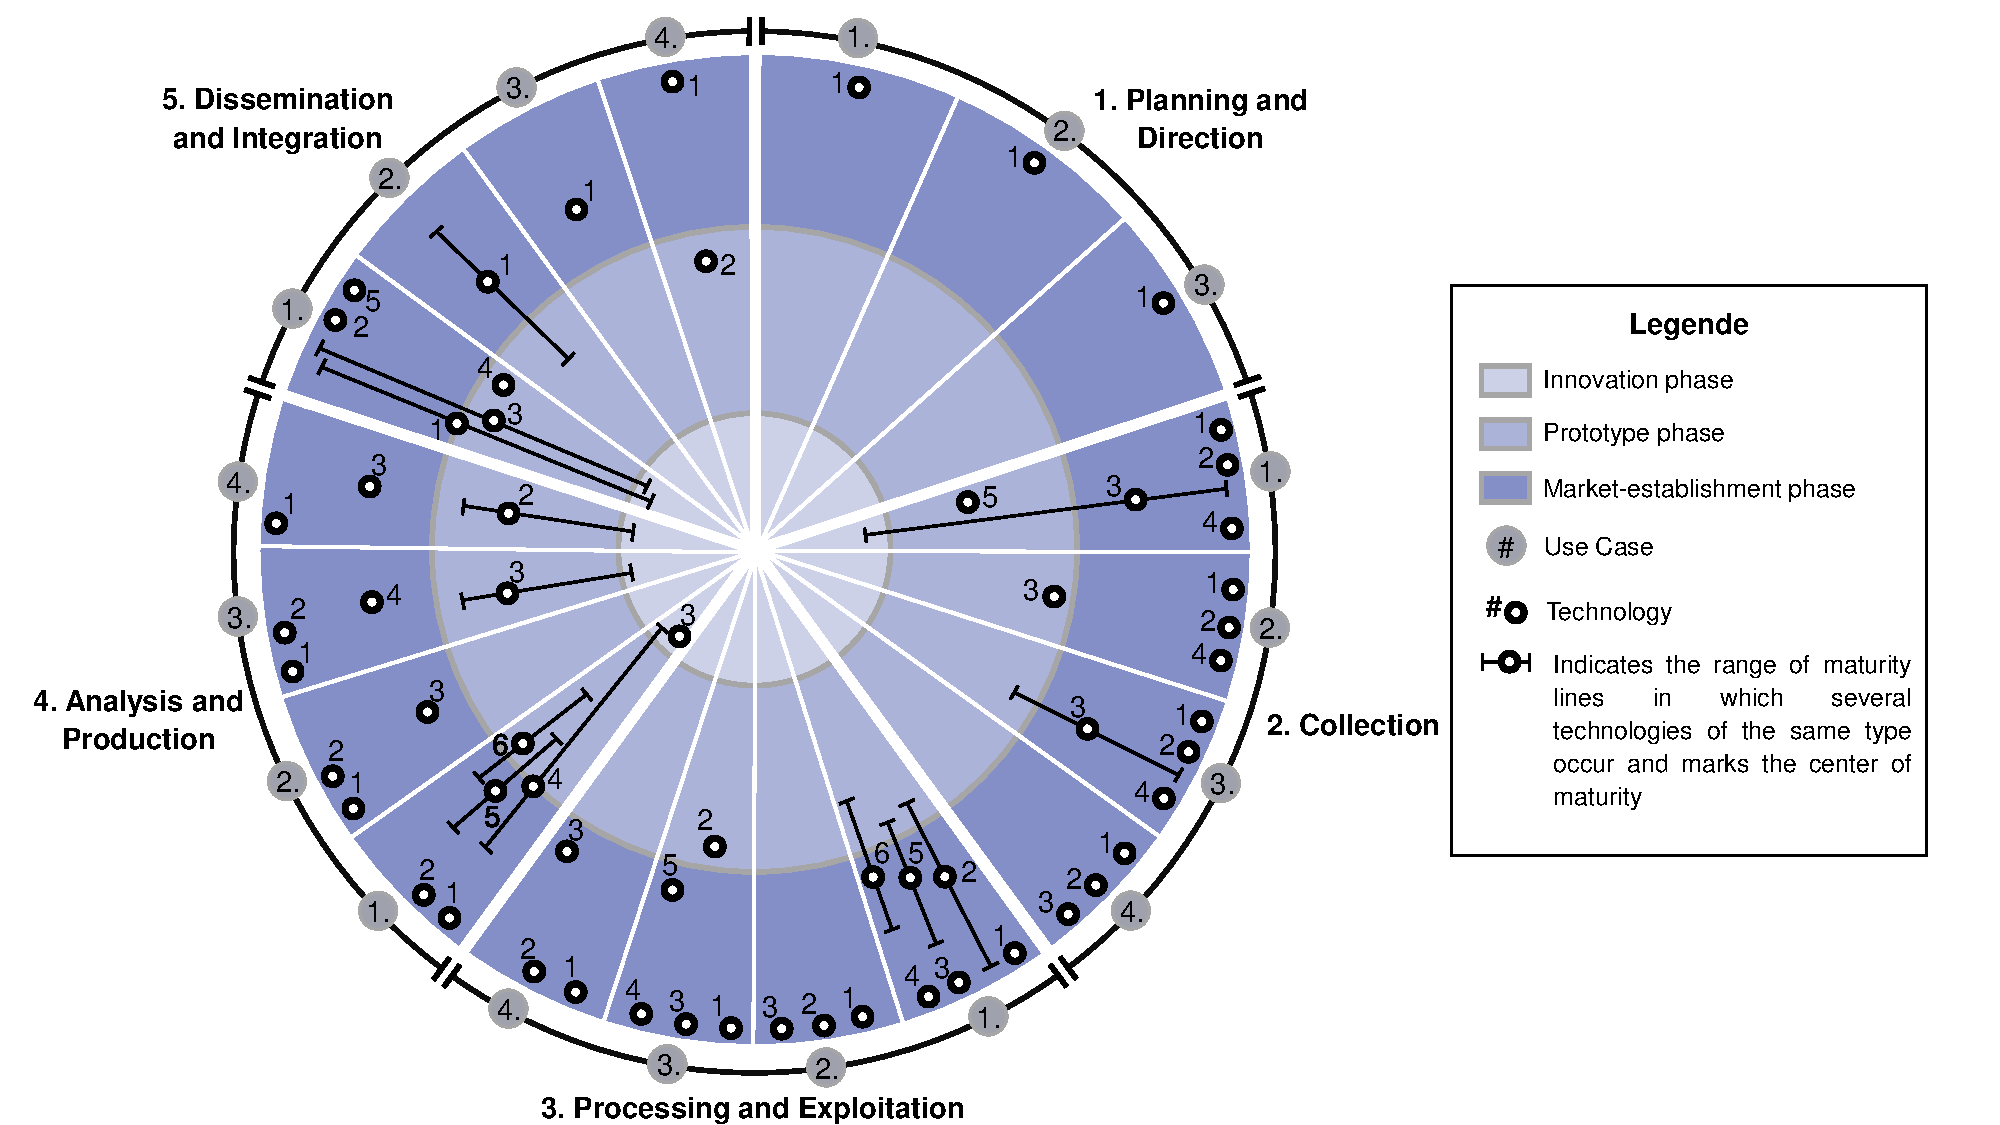
\includegraphics[width=\textwidth]{crop_Trendradar}
    \caption{Trend radar}
    \label{fig:trendradar}
\end{figure*}

\begin{figure*}[!thb]
    \centering
    \rotatebox{90}{%
        \begin{minipage}{\textheight}
            \centering
            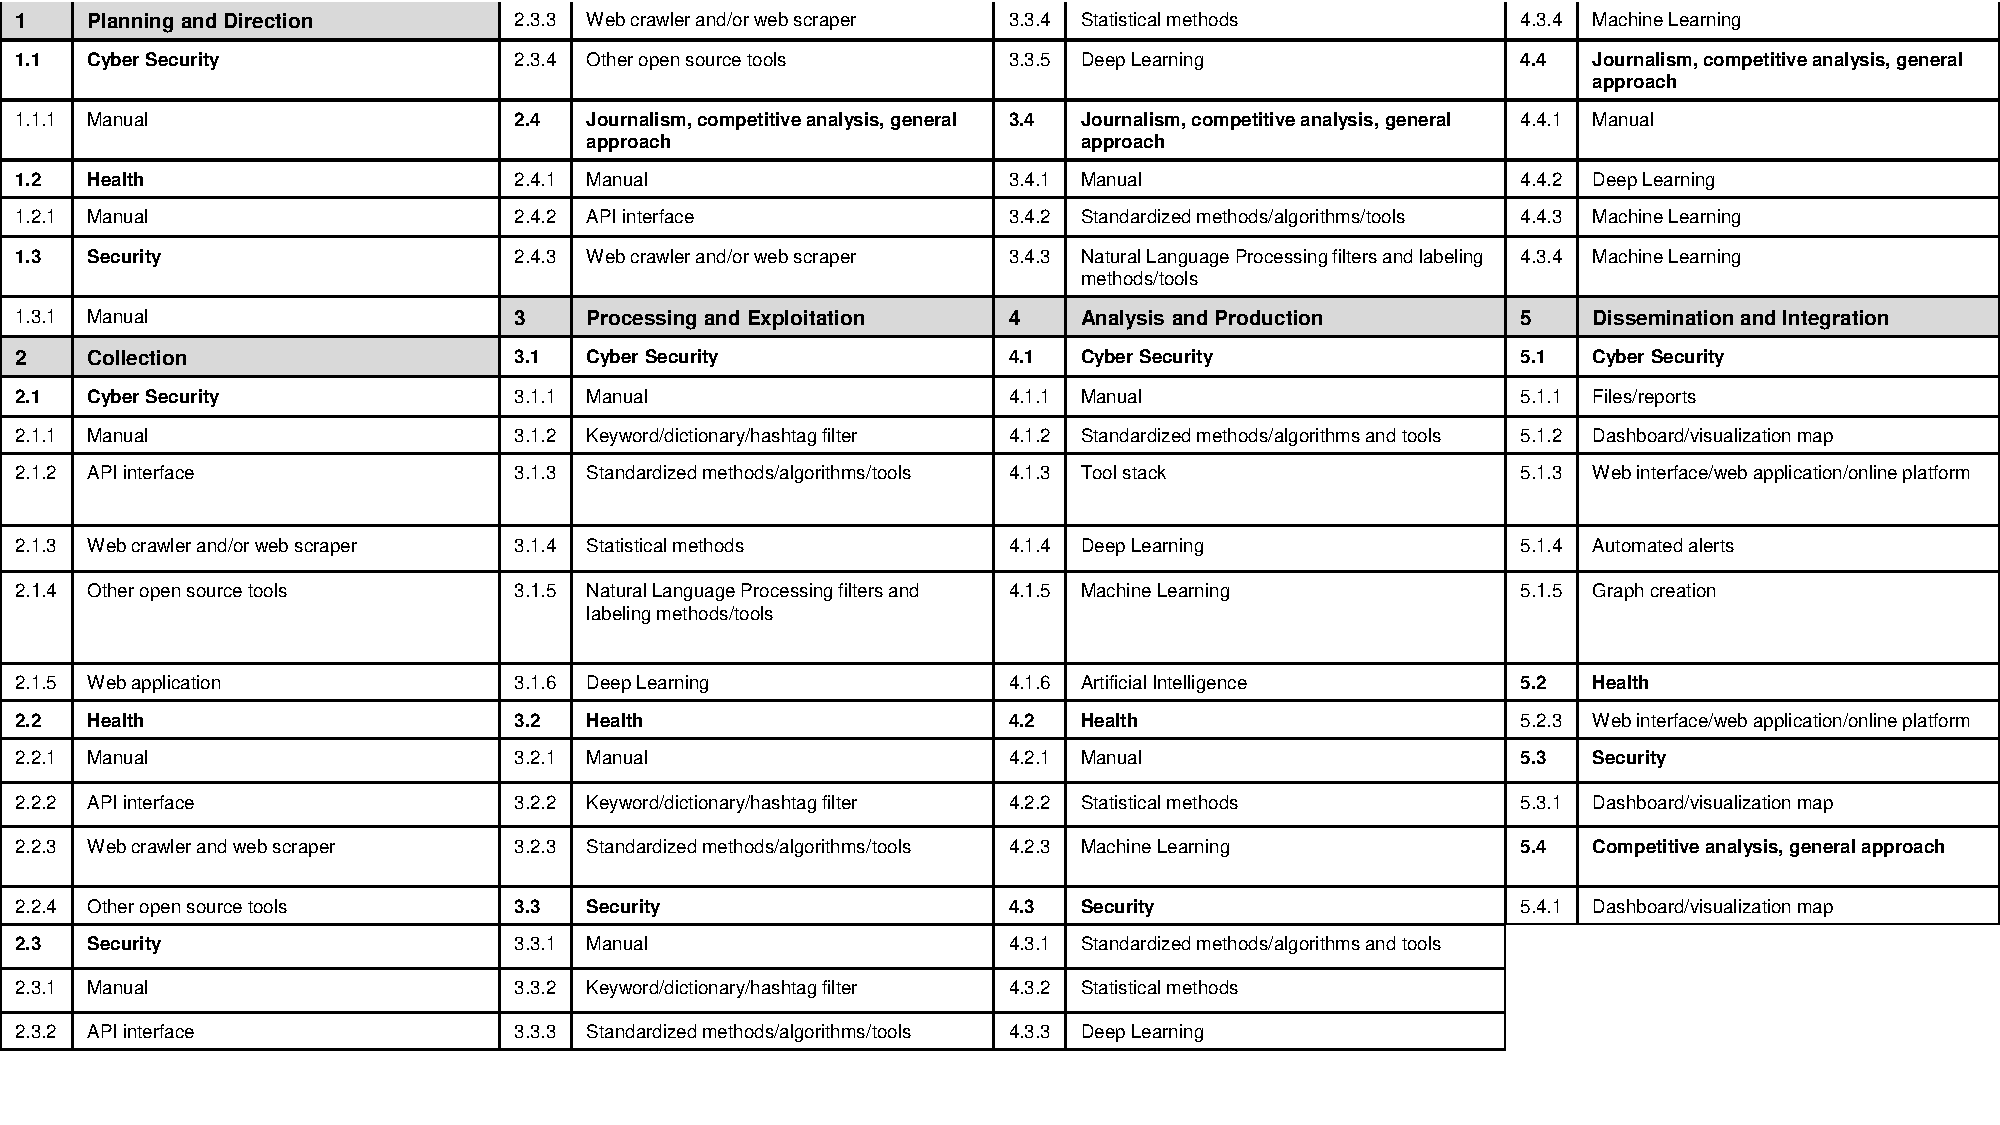
\includegraphics[width=\linewidth]{crop_Trendradar explanation}
            \caption{Trend radar explanation}
            \label{fig:trendradarexplanation}
        \end{minipage}%
    }
\end{figure*}

\subsection{Intelligence Cycle in Theory-Practice Comparison}

Studies could be attributed to each of the Intelligence Cycle phases. However,
none of the applications identified covers all phases in the sense of a third-generation
OSINT tool. Literature primarily focuses on the collection phase, followed by
the analysis and production phase and the processing and exploitation phase.
The dissemination and integration phase is covered by far the least after the planning
and direction phase.

These findings align with the experts' practical experiences. They regard the Intelligence Cycle as "state of the art" (cf. E3, 28.12.2023), but note different manifestations of the phases in praxis (cf. E4, 02.08.2023).
The planning and direction phase is often neglected, despite its crucial importance, leading to wasteful production (cf. E3, 28.07.2023). Conversely, OSINT is frequently associated solely with the collection phase,
resulting in subpar outcomes due to high volumes of low-quality data (cf. E1, 14.07.2023; E2, 19.07.2023; E3, 28.07.2023). The main reason for this is, that the Intelligence Cycle is operated by at least three groups of people. Firstly, the customers, usually located at the "decision-maker level", with a primarily legal professional background (cf. E2, 19.07.2023).
The second is the technician who carries out the data collection and processing (cf. E2, 19.07.2023; E3, 28.07.2023). Lastly, the analyst evaluates the data and creates the intelligence product (cf. E1, 14.07.2023). The process thereby is rarely transparent between the parties
(cf. E1, 14.07.2023; E2, 19.07.2023) and is rarely anchored at the organizational level (cf. E4, 02.08.2023). According to the experts, there is thus no third-generation
OSINT tool in use, at least not in German authorities. In addition, the collection focus is driven by concerns about missing vital information, which could later be revealed as publicly available (cf. E1, 14.07.2023).

\subsection{Use Cases in Theory-Practice Comparison}

Five main use cases emerged from the research: Cyber Security, Health, Security, Journalism,
and Competition Analysis. Cyber Security studies primarily focus on Open Source Cyber Threat
Intelligence (OSCTI), which involves collecting, monitoring, and analyzing publicly available
data to detect potential cyber threats \cite{Ahuja.2022,AlDmour.2023}.
Health applications mainly pertain to COVID-19, such as investigating the epidemic outbreak \cite{Kpozehouen.2020,Thamtono.2021}.
The security use case includes applications such as
analyzing violent behavior in public transport \cite{Nobili.2021}. The identified Journalism study examines the
Twitter activities of the OSINT journalists' association "Bellingcat" \cite{Bar.2023}. Competitive analysis
involves for example the performance classification of Chinese logistics companies \cite{Tao.2023}. Additionally, two
studies could be identified on general approaches to creating knowledge graphs on OSINF \cite{Hu.2023,Ma.2022}.

According to the experts, OSINT is applied in all authorities and has proven itself
in numerous use cases, even if not always explicitly labeled as such (cf. E2, 19.07.2023).
Most common cases are in cyber security/CTI (cf. E1, 14.07.2023; E2, 19.07.2023), as well as general security,
particularly with regard to the German Armed Forces, the (Federal) Intelligence Service,
the Ger­man do­mes­tic in­tel­li­gence ser­vices and the police.

\subsection{Technologies and Maturity Levels in Theory-Practice Comparison}

Except for the initial phase, automated technologies are utilized across all subsequent phases and use cases.
These technologies demonstrate considerable market maturity, yet manual activities remain prevalent.
The highest level of automation is observed in the CTI use case.

The most advanced automated technology in the collection phase is web crawlers and/or web scrapers.
Established technologies include "off the shelf" tools (cf. \cite{Middleton.2020}) and open source
solutions like "Tweepy," a Python library for Twitter crawlers (cf. \cite{Adewopo.2020,Tekin.2021}).
More advanced prototypes involve combining parallelized, recursive, source-specific web crawlers and scrapers for improved
data collection (cf. \cite{Jenkins.2021,Rajendran.2022}). Another method in the prototype phase is
"focused crawling", adapting the crawling path dynamically using a content-driven ML algorithm, BERT ("Bidirectional Encoder Representation from Transformers")
(cf. \cite{Kuehn.2023}). Technologies for crawling/scraping the dark web, like "Torsion" (cf. \cite{Sonawane.2022}),
were assigned to the innovation phase. The experts also note the increasing use of open source tools alongside manual work
(cf. E1, 14.07.2023; E3, 28.07.2023; E1, 14.07.2023). However, they consider traditional web crawling and scraping
outdated due to errors, implementation difficulties, and website resistance. Screenshot-based "web shooting" with
subsequent OCR (Optical Character Recognition) extraction is seen as more modern and robust (cf. E3, 28.07.2023).

NLP applications/methods such as "Topic Classifying," "Part-of-Speech Tagging", "Entity and Relation Annotation", and "Named Entity Recognition"
demonstrate high automation levels in the processing and utilization phase. Technologies commonly used include
the "Python NLTK Toolkit" \cite{Hubbard.2022} and the "Stanford CoreNLP Toolkit" \cite{Middleton.2020}.
Additionally, deep learning, particularly through "word embedding" using the "word2vec" algorithm, is prominent
\cite{Bai.2020,Pingle.2020,Shen.2020}. However, the experts note that
this phase within authorities predominantly involves manual work due to the irreplaceable domain knowledge of experts
(cf. E1, 14.07.2023; E2, 19.07.2023; E3, 28.07.2023). The degree of automation of technologies thus depends on the abstraction level.
Operational tasks, which often require specific individual information, show lower automation levels compared to long-term general strategic analyses
requiring extensive data (cf. E3, 28.07.2023).

The highest automation level is observed in the analysis and production phase, where AI, ML, and DL technologies are prevalent.
Under DL, vectorization algorithms can also be found. Particularly BERT algorithms in different versions are commonly utilized
(cf. \cite{Ma.2022,Chen.2023}). Furthermore, even under ML vectorization models such as BERT or
"Supervised Support Vector Machines" (SVM) (see e.g.:\cite{Iorga.2020}) are listed.
In addition, the algorithms "Random Forest", XGBoost ("eXtreme Gradient Boosting)",
lightGBM ("light Gradient Boosting Machine"), "Naive Bayes" and "logistic regressions" are particularly common.
Publications thereby often utilize multiple algorithms concurrently for performance comparison (e.g. \cite{Tao.2023})
or for layered analysis (e.g. \cite{Yang.2022}). AI technologies are generally less specified,
except for Dale et al. \cite{Dale.2023}, who developed a bidirectional recurrent neural network with
BiGur ("Bidirectional Gated Recurrent Unit") layers. Due to the modular use of publicly available models,
the technologies are mostly classified as market-ready. Despite the potential, practical work in this phase
largely relies on manual content analysis due to a lack of technological understanding and acceptance,
especially at the contractor/provider level in Germany (cf. E2, 19.07.2023; E3, 28.07.2023; E4, 02.08.2023). Furthermore,
ethical and legal barriers, such as GDPR (General Data Protection Regulation), hinder technology adoption
(cf. E2, 19.07.2023; E4, 02.08.2023). Additionally, security concerns in German authorities favor
standalone systems (cf. E2, 19.07.2023). If smart technologies are used, it is often only inofficially
(cf. E4, 02.08.2023). However, there's a need for modular, dynamically expandable
systems to keep pace with rapid advancements (cf. E1, 14.07.2023; E3, 28.07.2023; E4, 02.08.2023).
Nevertheless, human experience and specialization should not be outweighed, but rather a certain product quality
be ensured in a supportive manner. Yet, the revolutionary potential of large language models (LLM) cannot be estimated (cf. expert E4, 02.08.2023).

In the dissemination and integration phase, tools like "Power BI" \cite{Tao.2023}
are utilized to create dashboards and visualization maps. Furthermore, user interfaces,
web applications, and online platforms are developed, including Python GUIs,
specific browser applications \cite{Elmas.2022},
improved user interfaces and input masks for entire tool stacks \cite{Arjun.2020}.
Additionally, Technologies for generating automated alerts, particularly for cyber security risk assessments,
are prevalent \cite{Ahuja.2022}. Graph-based visualizations are also common, utilizing tools
/libraries like "Matplot," "Networkx," "Pygraphistry," or the "Neo4j-Browser" \cite{Middleton.2020}.
Except from the alerts, the retrieval of results is largely semi-automated and the technologies are in the
market establishment phase. No information on targeted user tests or a new development run involving
user feedback could thereby be found in any of the studies. The experts state that there is still very little
automation within the authorities during this phase. The final product is often only a PDF document,
an email or a verbal report (cf. E1, 14.07.2023), although in many cases no more is required (cf. E3, 28.07.2023).
However, outside of the OSINT topic, there are several automated tools, that could be transferred
to the authorities in this context (cf. E4 02.08.2023). Moreover, in practice, there is also a lack of
necessary feedback for product improvement (cf. E3, 28.07.2023).

\section{Discussion}

\subsection{Contributions and Implications}

The investigation into the existence of a robust, automated third-generation OSINT system
(cf. e.g: \cite{Ghioni.2023,PastorGalindo.2020,Yogish.2021})
leads to a negative conclusion, at least for Germany. Identified applications fall short of fully covering
the intelligence cycle, with significant gaps in the planning and direction phase,
followed by the dissemination and integration phase. Humans therefore remain the driving (analysis)
component. However, the finding by Pastor-Galindo et al. \cite{PastorGalindo.2020} that intelligent OSINT
concepts are not yet widespread cannot be confirmed either. Numerous intelligent tools available
on the market were identified in the other phases. Nevertheless, practical integration has so far
fallen short of the (theoretical) possibilities. Yet this finding likewise does not confirm the
thesis of Yogish et al. \cite{Yogish.2021} that automated, AI-driven solutions, largely eliminating
the human component, are inevitably required in every area of OSINT. Rather, the key research
question should be why proven, available applications whose support is needed have not
yet found widespread use, especially in intelligence authorities. In addition, the question of how the
first and last Intelligent Cycle phases, alongside the others, can be better supported technically
should be investigated.

Addressing these research questions entails resolving numerous underlying research gaps (RGs),
directly corresponding to the three key groups involved in the intelligence cycle. Primary among
these are the product customers. (RG1) Technologically, there's a deficiency in tools covering the
initial phase of the intelligence cycle, particularly in frameworks and tools for targeted requirements
definition and communication, which could alleviate the overemphasis on the collection phase \cite{Lowenthal.2020}.
(RG2) Moreover, concerning the final phase, there's a dearth of dissemination and integration mechanisms
tailored to authorities, largely due to insufficient user testing and iterative feedback incorporation.
However, established frameworks and the Intelligence Cycle itself underscore the indispensability of
consumer feedback for value-generating products \cite{DirectorofNationalIntelligence.2011,JointChiefsofStaffU.S.Army.2013,NorthAtlanticTreatyOrganization.2001} as it can significantly reduce data overload \cite{Gibson.2016} and enhance product credibility and quality \cite{Day.2016}.
(RG3) Furthermore, the future of OSINT systems hinges on modular concepts, yet only two studies have
been found on this (cf. \cite{Arjun.2020,Wright.2020}). (RG4) Accordingly, it's imperative to revamp
procurement procedures moving away from monolithic stand-alone setups. (RG5) Ensuring compliance with
ethical and legal principles at the client and customer level is vital for product adoption, necessitating robust legislative updates to establish appropriate frameworks \cite{Ghioni.2023,Wittmer.2022}.
This involves not only national but also international-level considerations, such as GDPR regulations
\cite{EuropeanParliament.2016,EuropeanCommission.18.08.2023}, taking into account not solely
individual but societal impacts \cite{Ghioni.2023}. To date, these topics remain underexplored \cite{Ghioni.2023,Wittmer.2022}. (RG6) Addressing these challenges necessitates a foundational level of technical understanding at decision-maker
levels, fostering openness to technology, and cultivating an information-sharing mindset, leveraging the public availability of information to transcend bureaucratic
barriers \cite{NorthAtlanticTreatyOrganization.2001}.

The analysts, comprising the second group, create the final
product and, at present, cannot be replaced by AI systems due to their extensive domain
knowledge \cite{Eldridge.2018,PastorGalindo.2020}. (RG7) However,
LLMs show promise in this realm, potentially becoming vital tools given their versatility
\cite{Radford.2023,Zhao.31.03.2023}. Yet, the use of such models in
application development could not be found. For the time being, cross-use case task
transferability can only be mapped to a limited extent with current learning algorithms
and is currently still subject to human cognition (cf. \cite{Schilling.2019,Ghioni.2023}.
Until then, the pursuit of the ideal symbiosis between humans and machines to bolster analysts
amid the deluge of data remains paramount \cite{Eldridge.2018}.

The third group, comprised of technicians, often handles the second and third phases of
the intelligence cycle independently (RG8). Technologically, there's a notable absence of
robust collection tools at this level to match the rapidly evolving media landscape (RG9).
Process-wise, coordination gaps with analysts pose a risk of excessive data collection.
Lowenthal \cite{Lowenthal.2020} suggests that data collection biases may stem from emotional or
lobby-driven factors, as it's seen as more enticing than its maintenance. Additionally,
the fear of overlooking pertinent information underscores the necessity for technological
tools to enhance transparency.

\subsection{Limitations and Future Research}

The first limitation relates to the fact that, due to a lack of clarity about the legal
and ethical basis \cite{Ghioni.2023,Unver.2018,Wittmer.2022},
it could not be verified whether only public sources \cite{NorthAtlanticTreatyOrganization.2002} were used
in the analyzed studies. It was also not verified whether the technologies meet the
legal and ethical requirements for the use of the information obtained
\cite{PastorGalindo.2020,Wittmer.2022}. The second
limitation stems from classification categories not fully aligning with the
MECE (Mutually-Exclusive-and-Collectively-Exhaustive) principle \cite{Lee.2018,Rasiel.1999},
particularly evident in the hierarchical dependency of AI, ML, and DL technologies. In addition,
the wording of the authors was followed for objective reproduction when identifying the technologies,
but the accuracy of the information was not reviewed in detail. Moreover, no fixed limits could be defined
for the volume category, as these were not recorded in uniform dimensions in the studies.
The third limitation concerns the limited sample size in expert interviews. Due to the
extremely difficult-to-access target group, the active user level and the decision-maker
level within the authorities were not interviewed. For improved intercoder reliability,
independent verification of the coding carried out by at least a second researcher
is also recommended \cite{Bogner.2002c,Glaser.2009,MAXQDA.16.03.2020}.
Lastly, the research structure, following the DSRM process, was executed linearly rather
than iteratively as recommended \cite{Peffers.2007}.

Nevertheless, the study furnishes future researchers with a robust knowledge base on OSINT
through a practice-validated trend radar. This facilitates an updated assessment of OSINT
trends and underscores the current research landscape. The study reveals two crucial
unanswered research questions and offers nine detailed research gaps for further exploration
in the field. Before addressing these questions, future researchers are advised
to validate them further. Utilizing the presented tools to reevaluate literature
categorization and update identified technologies is recommended. In addition, semantic
control and indexing methods (e.g. LLM) should be included. Due to the high dynamic of the research field,
it is also recommended to integrate news articles and scientific journals with shorter publication cycles.
Reassessing categories based on MECE criteria and conducting further interviews, including internationally
and with active authority members, is advisable. Employing methods like the Delphi technique to evaluate
trends and establish consensus is suggested \cite{Hader.2000}. Subsequent iterations of the design process and adjustments
to the trend radar, if necessary, should follow based on these results \cite{Peffers.2007,Sonnenberg.2012}.

\section{Conclusion}

In this paper, a practice-validated trend radar was developed that depicts current trends
in the field of OSINT through applied technologies. It serves as a comprehensive knowledge base,
allowing for contemporary evaluation and analysis of OSINT technologies as well as identifying research
gaps for future studies, penetrating the complex research field. Moreover, it serves as a guideline for practitioners. The radar
is adaptable to the evolving subject area and transferable to other intelligence disciplines.
Results reveal the absence of an automated third-generation OSINT system in Germany, highlighting the
need for technological support in the planning and direction as well as the dissemination and integration phases.
The research questions identified for future studies are therefore, why proven, available applications,
have not yet found widespread use, especially in the security authorities.
In addition, the question of how the first and last Intelligent Cycle phases, alongside the others,
can be better supported technically is to be investigated. The research gaps identified extend
not only to technology but in particular to the legal, administrative, political and
social sciences, necessitating interdisciplinary collaboration. Above all, a need to catch up is seen
in the non-technical research fields, responsible for creating the decisive prerequisites for technology
implementation.


% Fonts specification --- not shown as it doesn't exist in the Word document either. 

%\section{Fonts}

%A summary of fonts is provided in Table \ref{tab: fonts}. 

%\begin{table}[thb]
%\centering
%\caption{\label{font-table} Font guide. \vskip 3pt }
%\label{tab: fonts}
%\begin{tabular}{l|rl}
%\hline \bf Type of Text & \bf Font Size & \bf Style \\ \hline
%paper title & 14 pt &  \bf bold \\
%authors & 10 pt &  \underline{email} underlined \\
%abstract title & 12 pt &  \bf bold\\
%abstract text & 10 pt &  \it italic\\
%section titles & 12 pt & \bf bold \\
%subsection titles & 11 pt & \bf bold \\
%document text & 10 pt  & \\
%captions & 9 pt & \sansserifformat{\captionsize sans-serif, \bf bold} \\
%bibliography & 9 pt & \\
%footnotes & 8 pt & \\
%\hline
%\end{tabular}
%\end{table}


\section{References}


%Bibliography 

\bibliographystyle{ieeetr}
\bibliography{references}




\end{document}
